\documentclass[11pt]{article}
\usepackage[T1]{fontenc}
\usepackage{lmodern,amsmath,amssymb,graphicx,xcolor,booktabs,array,enumitem}
\usepackage[letterpaper,margin=0.78in]{geometry}
\usepackage[colorlinks=true,linkcolor=blue,urlcolor=teal]{hyperref}
\usepackage{fancyhdr}
\definecolor{ink}{HTML}{172C3B}
\definecolor{teal}{HTML}{087F82}
\definecolor{blue}{HTML}{265DAB}
\pagestyle{fancy}\fancyhf{}
\fancyhead[L]{\footnotesize OpenAI math: independent illustrated reading editions}
\fancyfoot[C]{\thepage}
\setlength{\headheight}{15pt}
\setlength{\parindent}{0pt}\setlength{\parskip}{7pt}
\setlength{\emergencystretch}{2em}
\hypersetup{pdfauthor={Independent explanatory edition prepared with OpenAI Codex}}
\begin{document}
\begin{center}{\LARGE\bfseries How many pairs of points can be exactly one unit apart?}\par\vspace{12pt}{\large An illustrated reader for the planar unit-distance upper bound}\par\vspace{16pt}Independent reading edition, October 14, 2026\end{center}
\section*{Start here}Place finitely many distinct points in the plane and connect pairs at distance exactly one. A square grid supplies many such pairs, but a cleverly arranged configuration might supply more. The problem asks for an upper bound valid for every configuration, not just the grid.

The source claims a fixed improvement below the exponent $4/3$. It argues by contradiction: if configurations approach that exponent arbitrarily closely, their incidence structure would force an impossible algebraic pattern. The route passes through probability laws, information, arithmetic height, and independent signs of square roots.

Those topics can sound remote from a picture of points. The diagrams below trace why each enters: circles encode unit pairs, sampling laws describe which local views are typical, height controls arithmetic size, and a rectangle of ratios packages the final obstruction. The small examples make these objects concrete without pretending to reproduce the full asymptotic contradiction.
\paragraph{Reading prerequisites.} Ordinary arithmetic is enough for the opening examples. Later chapters introduce the specialized vocabulary; checking every original proof requires additional study.\par\textbf{Attribution.} Original manuscript by OpenAI. Added explanations and figures prepared with OpenAI Codex. This is not an official revision or independent theorem validation.\par\href{https://github.com/openai/math/tree/1581d4cbdd69a0faf34b2089614fe2a814316a6a/preprints/A-power-saving-for-planar-unit-distances-September-23-2026}{Pinned original manuscript and citation}.\newpage\section*{The source claim, precisely}Theorem 1.1 states that there are absolute constants $C>0$ and $1\le\beta<4/3$ such that $u(n)\le Cn^\beta$ for every nonnegative integer $n$, where $u(n)$ is the largest possible number of unordered unit-distance pairs among $n$ distinct planar points. The source establishes existence of a fixed gap; it does not give a numerical value of that gap in this theorem.\paragraph{How to read this edition.} Each chapter gives one concrete illustration, then explains how it connects to the source. Captions identify toys and original constructions. Source anchors use the original manuscript\textquotesingle s section and page numbering. The expanded PDF places this guide before the complete unchanged original PDF, preserving the original page numbers and bibliography.\subsection*{Your route through the argument}\begin{enumerate}\item Count unordered pairs and exclude the diagonals
\item Turn distance equations into circle incidences
\item A random edge does not produce a uniform random vertex
\item Sharing a center creates dependence between neighbors
\item A rectangle cancels shared multiplicative factors
\item Independent square-root signs provide an obstruction
\end{enumerate}\paragraph{Verification scope.} The accompanying code checks the displayed finite examples and preserves original-file hashes. These checks do not replace the analytic, algebraic, asymptotic, or formal proof obligations in the source.\newpage\section*{Count unordered pairs and exclude the diagonals}
\begin{center}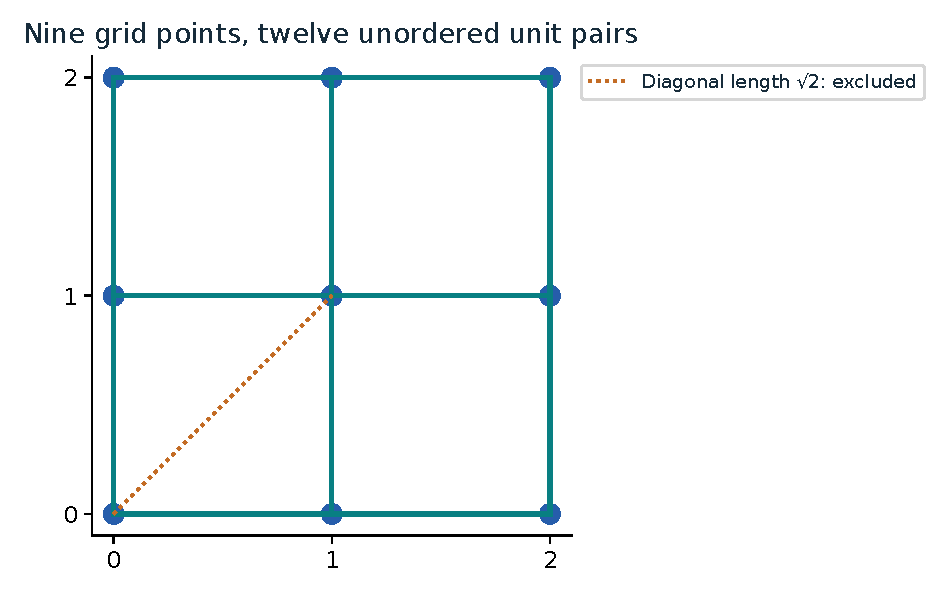
\includegraphics[width=\linewidth,height=2.35in,keepaspectratio]{figures/01-grid.pdf}\end{center}
{\small\color{teal}\textbf{Figure 1.} A 3$\times$3 integer grid has six horizontal and six vertical unit pairs. Diagonal neighbors have distance $\surd$2 and are excluded.\par}
There are $\binom92=36$ unordered pairs among nine points, but only twelve are at distance exactly one. In each of three rows there are two horizontal unit segments, giving six. The same count in columns gives six vertical segments. Diagonals are too long.

For a $k\times k$ grid, the same argument gives $2k(k-1)$ unit pairs among $n=k^2$ points. This is a construction lower bound: the maximum $u(n)$ is at least this count at those sizes. It is not an upper bound for arbitrary planar configurations.

The source counts unordered pairs in its headline theorem. Its incidence representation later uses ordered pairs and therefore counts each geometric unit segment twice when both copies of the point set are retained. A factor of two changes a constant, not the exponent, but keeping the conventions straight prevents mistaken numerical examples.

\paragraph{Why an exponent matters.} A bound $Cn^{4/3-\delta}$ with fixed $\delta>0$ eventually beats any fixed multiple of $n^{4/3}$. The statement concerns growth for large $n$, not a claim that the formula accurately predicts the maximum for nine points. Neither the constant nor an explicit gap is derived by the grid illustration.
{\footnotesize\color{blue}\textbf{Source anchor:} Section 1: u(X), u(n), and Theorem 1.1.\par}
\newpage\section*{Turn distance equations into circle incidences}
\begin{center}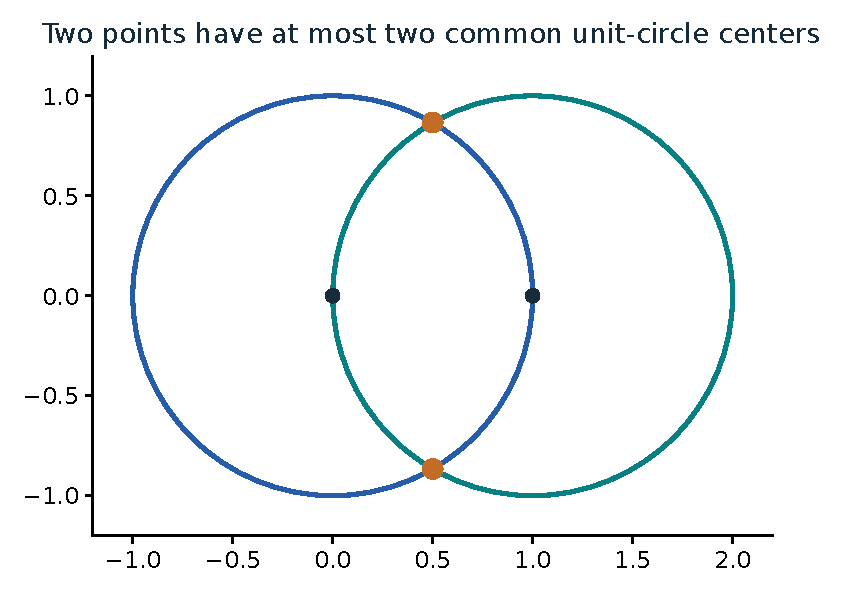
\includegraphics[width=\linewidth,height=2.35in,keepaspectratio]{figures/02-circles.pdf}\end{center}
{\small\color{teal}\textbf{Figure 2.} The unit circles centered at (0,0) and (1,0) meet at (1/2, ±$\surd$3/2). Those are the two possible centers one unit from both points.\par}
A point $p$ is one unit from a center $q$ precisely when it lies on the radius-one circle around $q$. This turns pair counting into point-curve incidence counting: count the occasions when a point lies on one of the circles.

Two distinct circles meet in at most two points. Reversing the viewpoint, two distinct points have at most two common unit-circle centers. In the example, solving $x^2+y^2=1$ and $(x-1)^2+y^2=1$ gives $x=1/2$, then $y=\pm\sqrt3/2$.

These bounded intersections help control the incidence graph. The source samples circles to cut the plane into regions meeting relatively few remaining circles, then keeps a graph piece with useful degree and expansion properties. Its handling of boundaries ensures that retained points are assigned consistently.

The elementary two-circle fact does not alone yield the claimed power saving. It supports the incidence reductions that make the later information and algebraic arguments possible. In particular, replacing the carefully retained graph by an arbitrary subset can change its sampling laws and destroy the properties used afterward.
{\footnotesize\color{blue}\textbf{Source anchor:} Section 2.2: point-circle incidences and the cutting construction.\par}
\newpage\section*{A random edge does not produce a uniform random vertex}
\begin{center}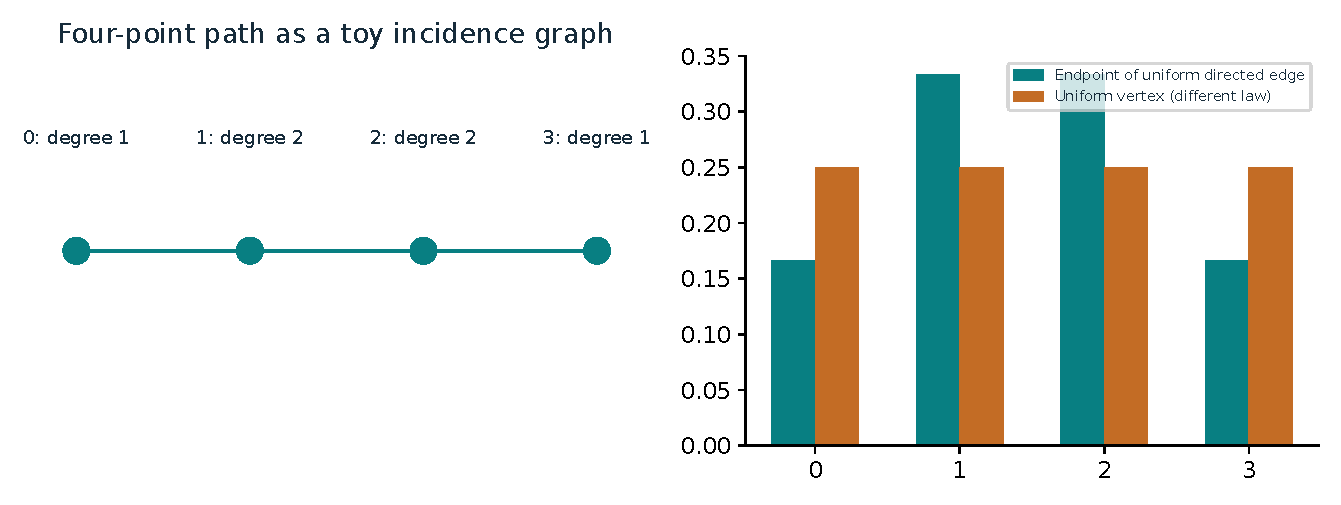
\includegraphics[width=\linewidth,height=2.35in,keepaspectratio]{figures/03-edge-law.pdf}\end{center}
{\small\color{teal}\textbf{Figure 3.} In a four-vertex path, the endpoint marginal of a uniformly chosen directed edge is (1,2,2,1)/6. The middle vertices are twice as likely as the endpoints.\par}
Choose one of the six directed edges of a four-vertex path uniformly, then look at its first vertex. A vertex occurs once for each incident edge, so its probability is proportional to its degree. The two end vertices have probability $1/6$ and the two middle vertices $2/6$.

Choosing one of the four vertices uniformly would instead give probability $1/4$ each. These experiments are different. An argument that resamples a vertex must preserve the required marginal, not substitute whichever distribution seems convenient.

The source consistently starts with a uniform retained edge. Point and center marginals are degree weighted. A prediction is sampled from the point marginal conditioned on agreeing with recorded test outcomes. Averaging over those histories preserves the original point marginal, an elementary conditional-probability fact with important consequences here.

The short-history argument must also keep a fresh test independent of the entire existing experiment. Allowing that test to depend on a prediction after seeing it would change the claim. The small path teaches the probability bookkeeping; it does not establish the source's low-information or prediction bounds for its dense incidence pieces.
{\footnotesize\color{blue}\textbf{Source anchor:} Sections 2-3: retained-edge law and conditional-copy prediction.\par}
\newpage\section*{Sharing a center creates dependence between neighbors}
\begin{center}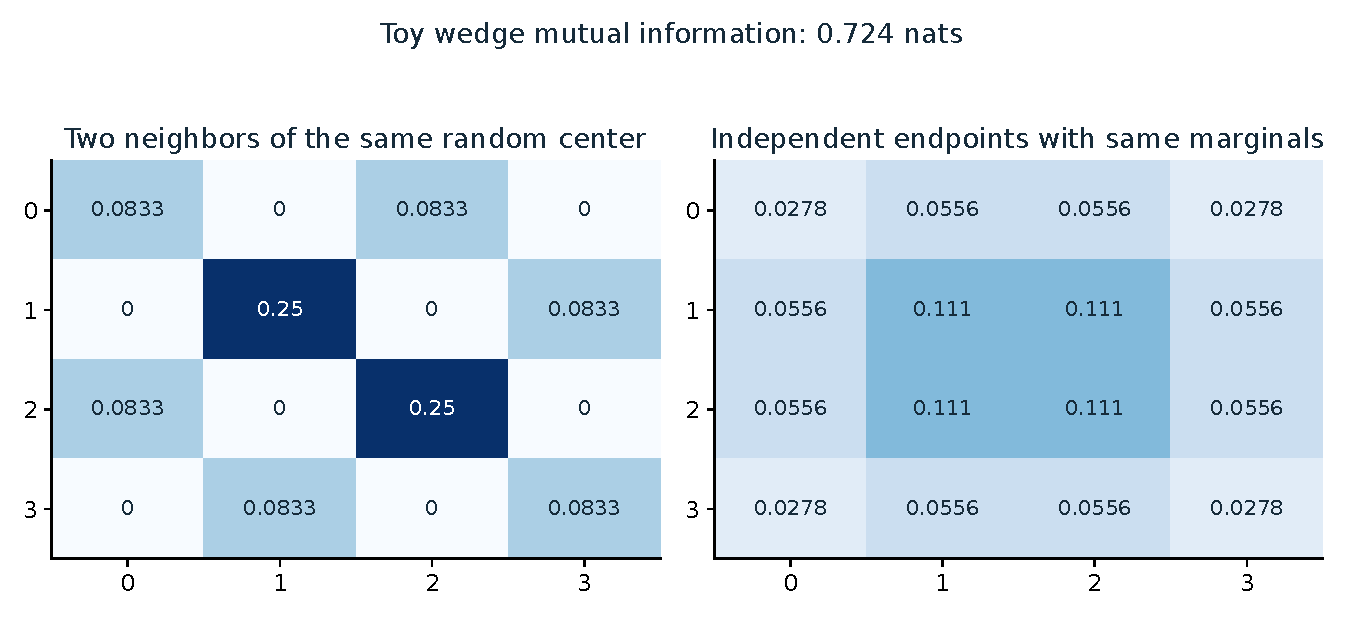
\includegraphics[width=\linewidth,height=2.35in,keepaspectratio]{figures/04-wedge.pdf}\end{center}
{\small\color{teal}\textbf{Figure 4.} Left: choose a degree-weighted center, then two neighbors independently conditional on that center. Right: choose endpoints independently from their common marginal. The matrices differ.\par}
A wedge is a two-edge path with a specified center. The endpoints are independent once that center is known, but usually not independent after the center is hidden. Both endpoints carry information about the same latent choice.

For the toy path, first choose center $c$ with probability $\deg(c)/6$, then select two neighbors with replacement, each uniformly from that center's neighbors. The joint probability is
\[P(i,j)=\sum_c\frac{\deg(c)}6\frac{A_{ci}}{\deg(c)}\frac{A_{cj}}{\deg(c)},\]
where $A$ is the adjacency matrix. Summing a row or column recovers the degree-weighted endpoint marginal. Repeated endpoints are allowed in this sampling experiment.

Mutual information compares this joint law with the product of its marginals. The expression is\[\sum_{i,j}P(i,j)\log\frac{P(i,j)}{P(i)P(j)},\]omitting zero terms. Zero would mean independence. The displayed toy has a positive value computed from its finite table.

The source proves a much more specific estimate, $o(\log t)$, for wedge endpoints in the retained configurations along its contradiction sequence. Our four-vertex calculation does not model that limit. It explains what quantity is being bounded and why conditional independence is not enough by itself.
{\footnotesize\color{blue}\textbf{Source anchor:} Section 2: wedge law and mutual information; Section 3 prediction.\par}
\newpage\section*{A rectangle cancels shared multiplicative factors}
\begin{center}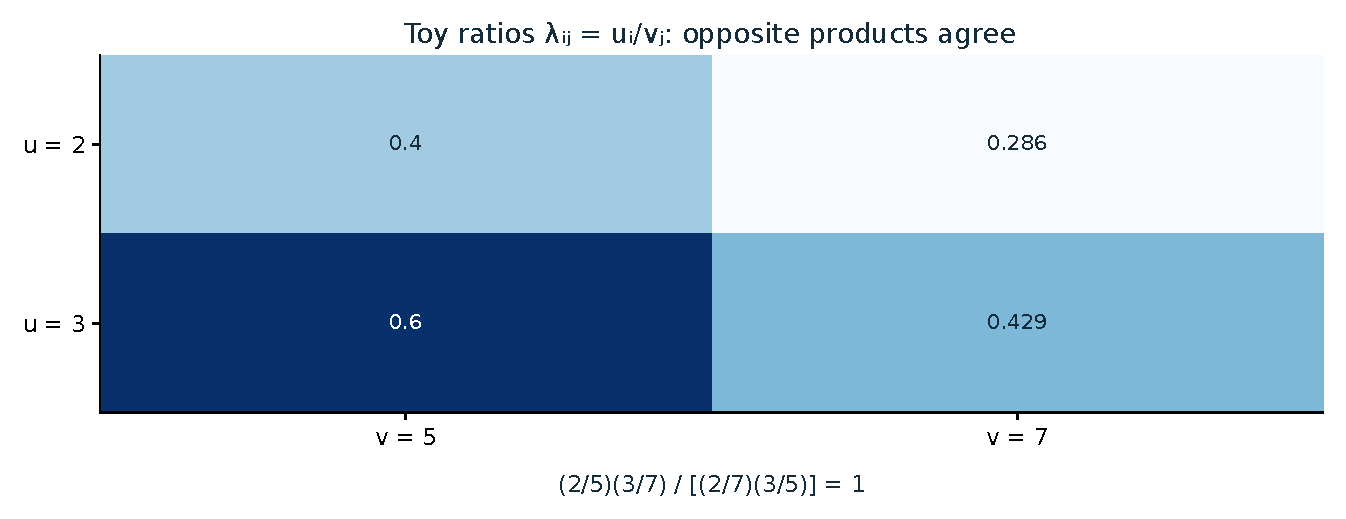
\includegraphics[width=\linewidth,height=2.35in,keepaspectratio]{figures/05-rectangle.pdf}\end{center}
{\small\color{teal}\textbf{Figure 5.} For the toy ratios $\lambda$$_i$$_j$=u$_i$/v$_j$, multiplying opposite corners and dividing gives one exactly. The source obtains small height for analogous rectangle products.\par}
Suppose a table has entries $\lambda_{ij}=u_i/v_j$. Around a two-by-two rectangle,
\[\frac{\lambda_{ij}\lambda_{i'j'}}{\lambda_{ij'}\lambda_{i'j}}=1.\]
Every row factor and every column factor cancels. Taking logarithms turns this into cancellation of alternating sums. This is why rectangles can detect whether pairwise quantities nearly split into endpoint contributions.

The source uses ratios of complex unit-edge jumps through selected centers. It builds a dense pair graph in which individual ratios have large arithmetic height, while every retained rectangle product has height small relative to a growing scale. The exact cancellation in our rational table is a teaching model for that comparison, not a unit-distance configuration realizing the source's hypotheses.

Arithmetic height measures algebraic size across all normalized absolute values of a number field. It is not Euclidean distance, decimal length alone, or the logarithm of one complex modulus. The product formula connects these different absolute values.

A key extraction step removes errors in a height-weighted measure before choosing a common height band. As in any weighted average, rare but very large errors cannot be dismissed by their probability alone.
{\footnotesize\color{blue}\textbf{Source anchor:} Sections 4-7: product formula, scale, and height-weighted rectangle extraction.\par}
\newpage\section*{Independent square-root signs provide an obstruction}
\begin{center}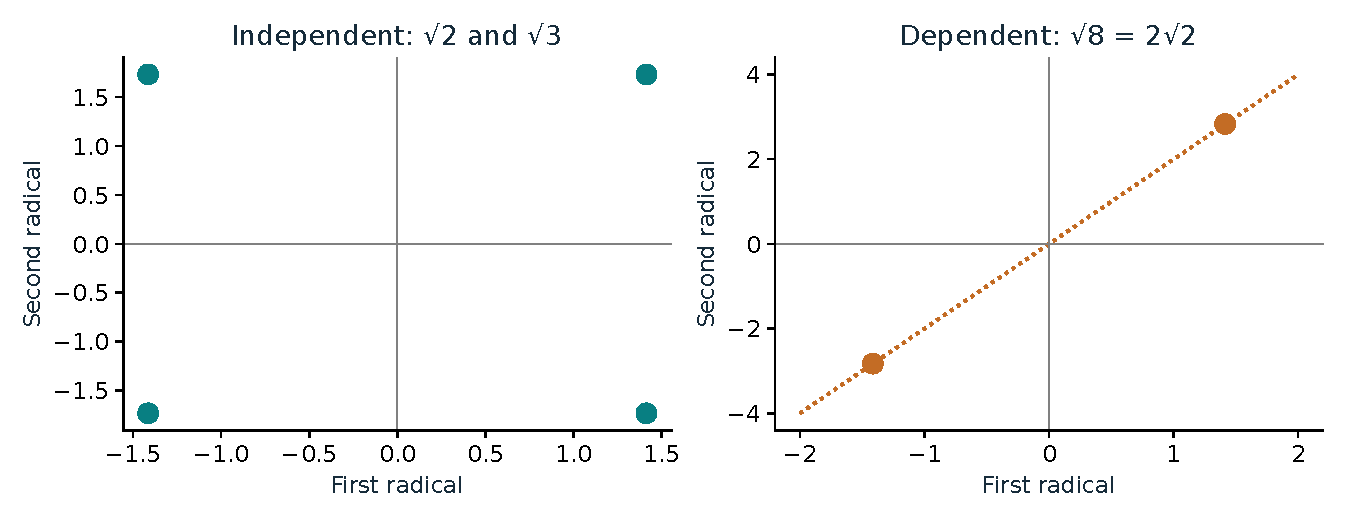
\includegraphics[width=\linewidth,height=2.35in,keepaspectratio]{figures/06-radicals.pdf}\end{center}
{\small\color{teal}\textbf{Figure 6.} Over the rationals, $\surd$2 and $\surd$3 admit four independent sign choices in their common field. For $\surd$2 and $\surd$8, the relation $\surd$8=2$\surd$2 allows only two linked choices.\par}
The expression $\sqrt2$ has two algebraic conjugates, $+\sqrt2$ and $-\sqrt2$. In the field containing both $\sqrt2$ and $\sqrt3$, their signs can be changed independently while fixing rational numbers. The four plotted points encode those choices.

By contrast, $\sqrt8=2\sqrt2$. Any transformation fixing rational numbers and preserving multiplication must flip those two radicals together. There are only two possibilities, on the displayed line. Writing two square-root symbols does not guarantee two independent signs.

In the final source argument, radicals arise from pair-distance identities. The proof constructs valuations that are odd on one radicand and zero on the others, ensuring the needed independence over the relevant coefficient field. It then changes an unused radical's sign in differentiated equations and obtains a contradiction. Excluding popular unit circles removes a geometric case that would interfere with that independence.

These rational examples explain the logic of independent versus linked radicals. They do not prove independence for the source's much larger field or its chosen points. Those algebraic and generic-position obligations are the core of Section 8.

The conclusion rules out all sequences approaching the exponent $4/3$ closely enough, which yields an unspecified fixed power saving.
{\footnotesize\color{blue}\textbf{Source anchor:} Section 8: generic configurations, valuations, and radical sign changes.\par}
\newpage\section*{A vocabulary you can return to}
\paragraph{Incidence}A point lies on a specified curve.
\paragraph{Degree-weighted marginal}A vertex probability proportional to the number of incident edges.
\paragraph{Wedge}Two edges sharing a sampled center.
\paragraph{Mutual information}Relative entropy of a joint distribution from the product of its marginals.
\paragraph{Arithmetic height}A measure of algebraic size using all normalized absolute values.
\paragraph{Independent radicals}Square roots whose signs can be changed independently over a specified base field.
\section*{What this edition checks}The checked grid, probability tables, and rational rectangle identity are educational examples. This guide does not verify the cutting bounds, prediction theorem, height extraction, generic-position argument, or radical-independence proof. No numerical value of the source's exponent improvement is invented, and no comparison with a claimed current best lower bound is needed for this reading edition.
\paragraph{A useful self-test.} Explain what each plotted quantity counts, which examples are illustrative, and where the source needs a statement for every input or every sufficiently large size. If a picture seems to establish the full theorem by itself, revisit its caption and source anchor.\paragraph{Sources and reuse.}\href{https://github.com/openai/math/tree/1581d4cbdd69a0faf34b2089614fe2a814316a6a/preprints/A-power-saving-for-planar-unit-distances-September-23-2026}{A power saving for planar unit distances}, OpenAI. Original bibliography and manuscript-specific citation are included with the source. Source snapshot: \texttt{1581d4cbdd69}. This derivative is distributed under Apache-2.0 with the original attribution; see the repository LICENSE and NOTICE.\end{document}